% !TeX root = ./report.tex

本章将对 AGV 地图编辑器的功能进行详细的说明,将展示本软件完成的图例以及相应的流程、代码说明。本软件使用 Visual Studio 2017 进行开发,理论上可以使用 2017 以及 2019 版的 Visual Studio 进行编译。

\begin{figure}[H]
  \centering
  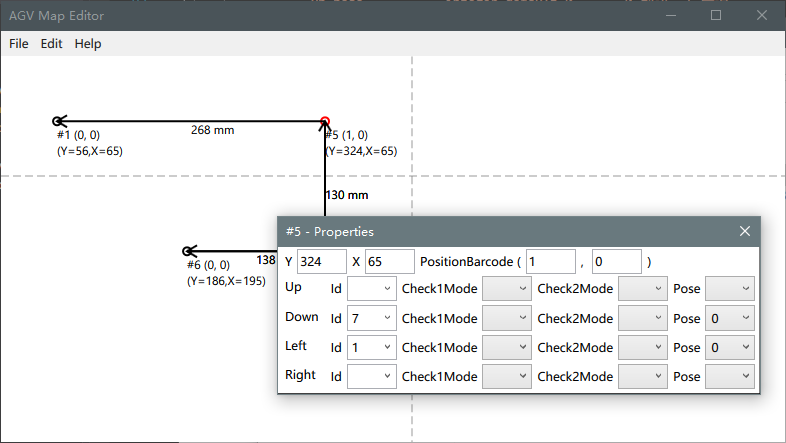
\includegraphics[width=0.8\textwidth]{assets/mainview.png}
  \caption{软件主界面}
  \label{fig:mainview}
\end{figure}

双击 Editor.exe 打开本软件。本软件的界面都是通过在 Visual Studio 中编写 XAML 代码实现的。主界面如上图,有菜单栏、地图编辑区域、属性窗口三个主要功能区。

\section{启动}

首次启动本程序时,会自动打开一个文件选择框选择将要打开的数据库文件,默认为 \texttt{MapData.db},如果文件不存在则会在第一次保存(见下)时自动创建。

\begin{figure}[H]
  \centering
  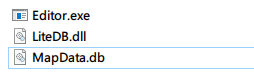
\includegraphics[width=0.4\textwidth]{assets/explorer.png}
  \caption{至少保存过一次后的程序文件夹}
  \label{fig:explorer}
\end{figure}

\section{创建坐标点}

移动鼠标,可以看到两条虚线分别对齐到鼠标的 XY 坐标上。此时在某一空白处双击即可在对应位置创建新的坐标点。

\begin{figure}[H]
  \centering
  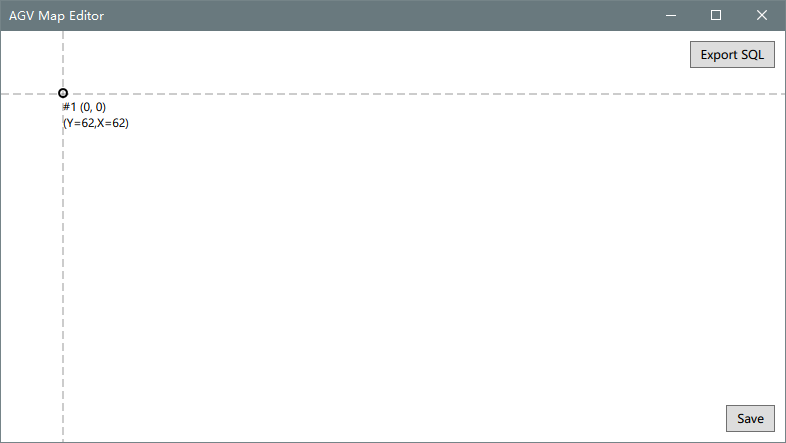
\includegraphics[width=0.8\textwidth]{assets/dbclick.png}
  \caption{在空白处双击后的界面}
  \label{fig:dbclick}
\end{figure}

坐标点的 ID 是自动分配的,不可以修改;XY 坐标赋值为鼠标位置,剩下的属性全都默认赋值为 0。坐标点被选中时,颜色变为红色。

\subsubsection{相关代码}

\begin{lstlisting}[language=cs]
private void Window_MouseDoubleClick(object sender, MouseButtonEventArgs e) {
    if (/* 是在空白处按下的 */) {
        Map.Add(Cur = new Coord { X = CurX, Y = CurY });
        foreach (Coord c in Map) c.Update(ic, OffsetX, OffsetY);
        NeedSync = true;
    }
    // ... 其他逻辑 ...
}
\end{lstlisting}

\section{删除坐标点}

按下 \texttt{Delete} 或通过菜单上的 Edit-Delete 即可删除当前被选中的坐标点,但用掉的编号不会再次变得可用。需要注意的是,删除时要记得将与其关联的连线一同删除,下面通过一个流程图来说明这一点。

\subsubsection{基本流程}

\begin{figure}[H]
    \centering
    \includegraphics[width=0.38\textwidth]{assets/impl-1.pdf}
    \caption{删除坐标点流程}
    \label{fig:impl-1}
\end{figure}

\subsubsection{相关代码}

\begin{lstlisting}[language=cs]
private void Ic_KeyUp(object sender, KeyEventArgs e) {
    if (e.Key == Key.Delete) {
        if (/* 当前有点被选中 */) {
            // 删除该点(数据)
            Map.Remove(LastCur);
            // 删除与这个点相连的箭头
            foreach (Coord c in Map) {
                if (c.Up == LastCur) c.Up = null;
                if (c.Down == LastCur) c.Down = null;
                if (c.Left == LastCur) c.Left = null;
                if (c.Right == LastCur) c.Right = null;
            }
            // 删除该点(视图)
            LastCur.Remove(ic);
            LastCur = Cur = null;
            NeedSync = true;
        }
        RefreshMap();
    }
    // ... 其他逻辑 ...
}
\end{lstlisting}

\section{拖动坐标点}

直接在某个坐标点上按下鼠标左键,然后拖动即可,该点的 XY 坐标会跟着改变。如果勾上了 Edit-Sync Next Points(如图 \ref{fig:sync}),其指向的其他点也会跟着移动。

\begin{figure}[H]
  \centering
  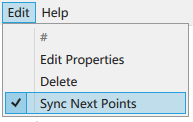
\includegraphics[width=0.4\textwidth]{assets/sync.png}
  \caption{同步移动它指向的其他点}
  \label{fig:sync}
\end{figure}

\subsection{拖动递归处理}

\begin{algorithm}[H]
  \caption{递归移动坐标点算法}
  \begin{algorithmic}[1]
    \Procedure{RecurUpdateNextCoords}{$cur, dx, dy$}\Comment{移动 cur 及它指向的其他点}
    \State $cur.X \gets cur.X + dx$ and $cur.Y \gets cur.Y + dy$\Comment{移动当前点}
    \If{$cur.Right$ 不为空}\Comment{递归处理右点}
      \State RecurUpdateNextCoords($cur.Right, dx, dy$)
    \EndIf
    \If{$cur.Down$ 不为空}\Comment{递归处理下点}
      \State RecurUpdateNextCoords($cur.Down, dx, dy$)
    \EndIf
    \EndProcedure
  \end{algorithmic}
\end{algorithm}

默认情况下,拖动时会自动``吸附''到其他坐标点的四方向上,这时按住 Ctrl 可以取消吸附。

\section{创建箭头}

在某一坐标点上按住鼠标右键然后拖动到另一个坐标点上,就会创建出对应的箭头。不可以从自己拖动到自己。

\section{拖动画布}

在空白处按住鼠标右键然后拖动,整个画布会跟着一起移动。

以上三个功能都涉及到鼠标移动,因此代码细节上我们选择将其实现在一起,其流程大致如下:

\subsubsection{基本流程}

\begin{figure}[H]
    \centering
    \includegraphics[width=0.85\textwidth]{assets/impl-2.pdf}
    \caption{移动鼠标时触发的流程}
    \label{fig:impl-2}
\end{figure}

\section{修改坐标点属性}

在一个坐标点上双击,即可打开``属性''窗口。

\begin{figure}[H]
  \centering
  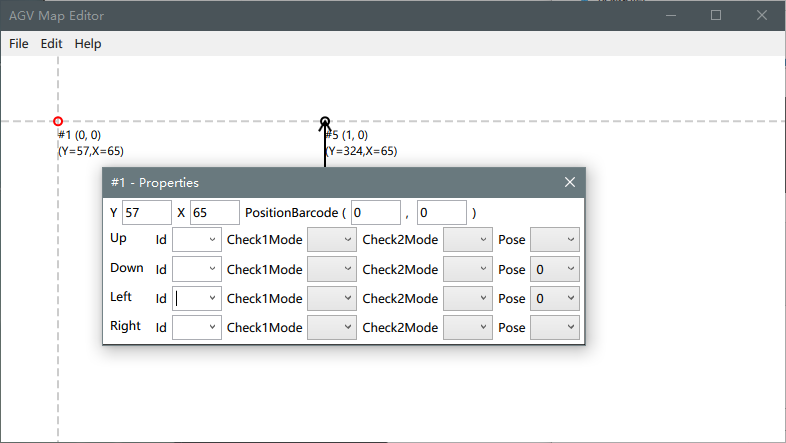
\includegraphics[width=0.8\textwidth]{assets/prop.png}
  \caption{``属性''窗口}
  \label{fig:prop}
\end{figure}

接下来我们尝试给 \#1 坐标点加一个指向 \#5 的路径,在 Right Id 下拉框中选中 5:

\begin{figure}[H]
  \centering
  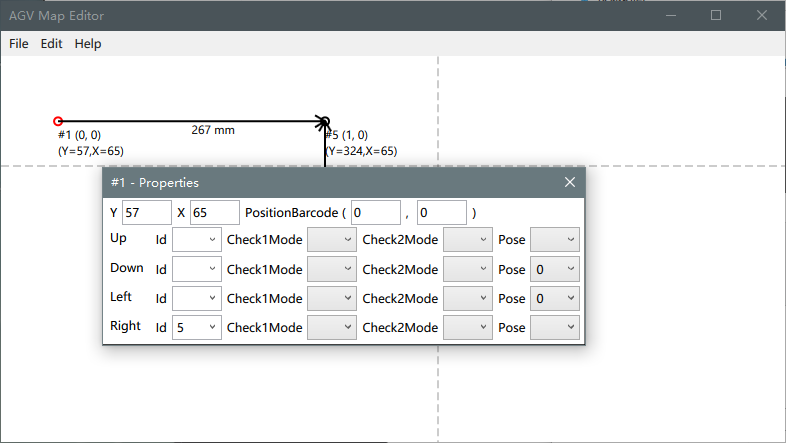
\includegraphics[width=0.8\textwidth]{assets/prop2.png}
  \caption{``属性''窗口}
  \label{fig:prop2}
\end{figure}

可以看到界面立刻产生了变化。这是因为为了使操作更方便,我将属性编辑功能设计并实现为直接写回软件内存的形式,这大大简化了操作,代价是代码量也增加了。现代的许多 UI(用户交互)设计都是这么做的,例如 Windows10 的``设置''功能等。

\subsubsection{相关代码}

\begin{lstlisting}[language=cs]
public Coord Coord {
  get => Coord_;
  // 读取坐标点数据到界面上
  set {
    Coord_ = null;
    X.Text = ((int)value.X).ToString();
    Y.Text = ((int)value.Y).ToString();
    I.Text = value.I.ToString();
    J.Text = value.J.ToString();
    if (value.Up != null) {
      for (int i = 1; i < UpId.Items.Count; i++) {
        if (Ids[i - 1] == value.Up.Id) {
          UpId.SelectedIndex = i;
          break;
        }
      }
      UpCheck1Mode.SelectedIndex = (value.M_Up & 0b01110000) >> 4;
      UpCheck2Mode.SelectedIndex = (value.M_Up & 0b00001110) >> 1;
      UpPose.SelectedIndex = value.M_Up & 0b00000001;
    } else {
      UpId.SelectedIndex = 0;
    }
    // ... 其他方向 ...
    Coord_ = value;
  }
}
private List<Coord> Map;
private int[] Ids;
// 直接写回软件内存
// 更新界面数据到坐标点本身
private void X_TextChanged(object sender, TextChangedEventArgs e) {
  if (Coord_ == null) return;
  if (Int32.TryParse(X.Text, out int _x))
    Coord_.X = _x;
  else
    X.Text = ((int)Coord_.X).ToString();
}
// 其他控件事件代码...
\end{lstlisting}

篇幅有限,代码均做了大量精简。

\section{保存到数据库}

点击文件菜单的``保存''按钮,即将数据写入数据库文件。

\begin{figure}[H]
  \centering
  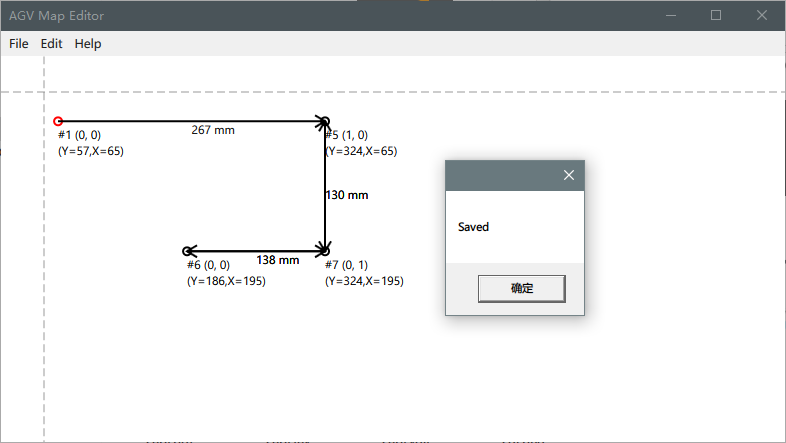
\includegraphics[width=0.8\textwidth]{assets/save.png}
  \caption{保存成功对话框}
  \label{fig:save}
\end{figure}

\subsubsection{相关代码}

\begin{lstlisting}[language=cs]
private void Sb_Click(object sender, RoutedEventArgs e) {
    // 生成部分必要数据
    foreach (Coord c in Map) c.UpdateNeighbours();
    // 写入数据库文件
    using (LiteDatabase db = new LiteDatabase(FileName)) {
        db.DropCollection("map");
        LiteCollection<Coord> map = db.GetCollection<Coord>("map");
        map.EnsureIndex(c => c.Id);
        map.InsertBulk(Map);
    }
    // 提示已保存
    MessageBox.Show("Saved");
    NeedSync = false;
}
\end{lstlisting}

\section{导出 SQL}

点击文件菜单的``导出 SQL''按钮,即将数据输出成 SQL 语句的形式。

\begin{figure}[H]
  \centering
  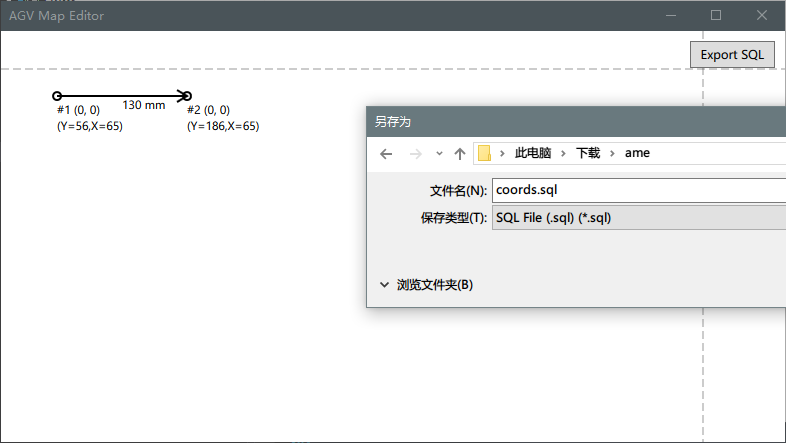
\includegraphics[width=0.8\textwidth]{assets/export.png}
  \caption{导出到 SQL 文件对话框}
  \label{fig:export}
\end{figure}

按确定后会在目标位置生成 SQL 文件,里面包含了创建和插入表的 SQL 语句。各个数据库的 SQL 是不一样的,这里选择生成的是 Sqlite 语法的 SQL,由于其简单的数据类型等特性,将其通过文本替换等方式直接转成其他数据库支持的 SQL 是相对容易的。

\begin{figure}[H]
  \centering
  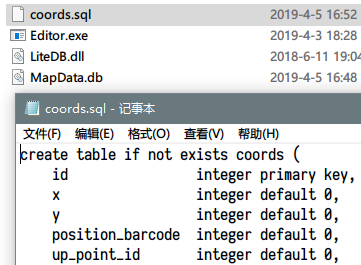
\includegraphics[width=0.5\textwidth]{assets/sql.png}
  \caption{SQL 文件内容预览}
  \label{fig:sql}
\end{figure}

\subsubsection{相关代码}

\begin{lstlisting}[language=cs]
// 生成一条插入语句
public string ToSql => $@"insert into coords values (
    {Id}, {(int)X}, {(int)Y}, {I * 10000 + J},
    {UpId}, {(M_Up & 0b01110000) >> 4},
    {(M_Up & 0b00001110) >> 1}, {(M_Up & 0b00000001)},
    {DownId}, {(M_Down & 0b01110000) >> 4},
    {(M_Down & 0b00001110) >> 1}, {(M_Down & 0b00000001)},
    {LeftId}, {(M_Left & 0b01110000) >> 4},
    {(M_Left & 0b00001110) >> 1}, {(M_Left & 0b00000001)},
    {RightId}, {(M_Right & 0b01110000) >> 4},
    {(M_Right & 0b00001110) >> 1}, {(M_Right & 0b00000001)}
)";

private void Es_Click(object sender, RoutedEventArgs e) {
    // 拼接 SQL 代码
    StringBuilder builder = new StringBuilder(Coord.ToTableSql);
    foreach (Coord c in Map) {
        builder.Append(c.ToSql);
        builder.Append(';');
    }
    string result = builder.ToString();
    // 询问保存位置
    SaveFileDialog dialog = new SaveFileDialog {
        FileName = "coords",
        DefaultExt = ".sql",
        Filter = "SQL File (.sql)|*.sql|Text documents (.txt)|*.txt"
    };
    // 如果确认保存,写入文本文件
    if (dialog.ShowDialog() == true) {
        File.WriteAllText(dialog.FileName, result);
    }
}
\end{lstlisting}
